\chapter{Formalism}
\section{State Vector}
\begin{itemize}
\item In Quantum Mechanics, we start with an object called the state vector $\ket{\psi}$. All the information about the system is contained in it. 
\item The position basis representation of the state vector is called the wavefunction $\psi (\vec{x}, t) = \braket{x}{\psi}$.
\item If we wish to know about a particular physical measurable such as an object's position of momentum, we can extract this information from the State vector by means of acting on with an Operator that corresponds to the measurable quantity.
\end{itemize}
\subsection{Admissibility Conditions for a Wavefunction}
A physically relevant wavefunction must be:
\begin{itemize}
\item Continuous i.e. no singularities in it's topology
\item Smooth i.e. a Taylor expansion for it exists
\item Quadratically integrable with the integral being single valued i.e. finite everywhere and $\psi \rightarrow 0$ as $r \rightarrow \infty$
\item Forming an orthonormal set
\item Satisfying the boundary conditions of the quantum mechanical system it represents
\end{itemize}
\section{Observables}
\begin{itemize}
\item Observable quantities such as position and momnetum c
\end{itemize}

\section{Time Evolution}
\subsection{Schrodinger Picture}
Where\\
If we consider the Schrodinger picture i.e. the state vector evovles with time whereas the Observables are in a loose sense eternal. The time evolution of the state vector is given by the Schrodinger equation:
\begin{equation}
	i \hbar \frac{\partial \ket{\psi}}{\partial t} = \hat{H} \ket{\psi}
\end{equation}
Or,
\begin{equation}
	i \hbar \frac{\partial \psi}{\partial t} = \hat{H} \psi
\end{equation}
in terms of the Wavefunction. Where, $\hat{H}$ is the Hamiltonian operator, which can be expressed as:
\begin{equation}
	\hat{H} = -\frac{\hbar^{2} \nabla^2}{2m} + V(\vec{x})
\end{equation}
for a free particle. 

\subsection{Heisenberg Picture}

\section{Measurement}
Measurement is defined as a form of time-evolution that is non-unitary and non-deterministic. 
According to Born's rule
\begin{equation}
	\int_{a}^{b} \abs{\psi(\vec{x}, t)}^{2} dx = \text{Probability of finding the particle at a time t between positions a and b}
\end{equation}
Thus, . Physically speaking this lends a kind of indeterminancy to the wavefunction. We can only speak of probabilities. Therefore, we can only , this brings to the measurement hypothesis, that is the State vector evolves to the state corresponding to the measurement being made. And unlike the Schrodinger equation, this evolution is non-deterministic. This tension is often called the "measurement problem", i.e. why is the measurement of an observable a special process distinct from others? Several theories and models claim to have resolved this, but we shall save that discussion for another time. We will fully focus on understanding the theory of Quantum Mechanics in a pragmatic lens before we question its foundations (although the converse isn't necessarily a bad thing, it isn't the purpose of this manuscript however).

\section{Summary of Postulates}
\begin{figure}
	\centering
	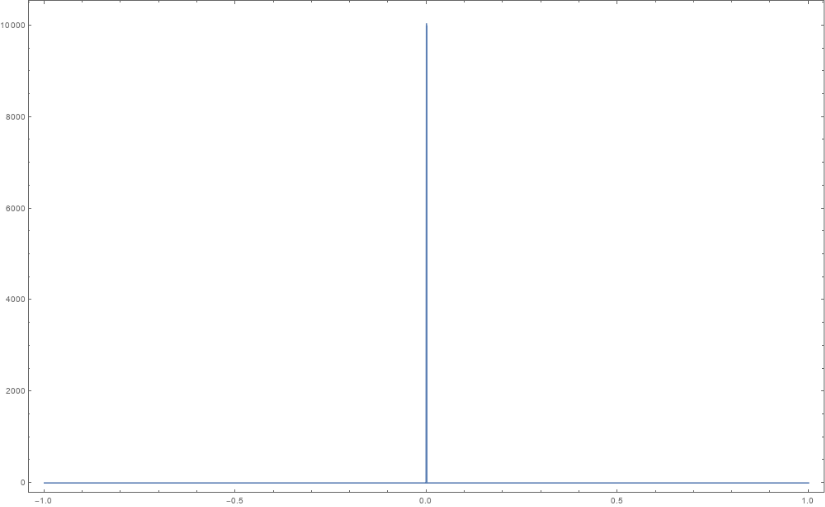
\includegraphics[scale=0.5]{delta-distribution.png}
	\caption{A Plot of $\delta(x)$}
\end{figure}
\section{Normalization}
Normalization is a process through which we ensure that,
\begin{equation}\label{norm}
	\int_{- \infty}^{\infty} \abs{\psi(\vec{x}, t)}^{2} dx = 1
\end{equation}
This is a natural consequence of Born's rule, we simply want all the probabilities to add up to 1. Thus, to rule out any other absurd scenarios, we make a ruling that non-Normalizable and non-square integrable Wavefunctions are unphysical.\\
We can also prove that once normalized, the wavefunction always remains normalized, we start by differentiating equation (\ref{norm}) with respect to time\\
$$\frac{d}{dt} \int_{- \infty}^{\infty} \abs{\psi(\vec{x}, t)}^{2} dx = \frac{\partial}{\partial t}\int_{- \infty}^{\infty} \abs{\psi(\vec{x}, t)}^{2} dx$$
Dealing with the term inside the integral,
$$ \frac{\partial}{\partial t}\abs{\psi(\vec{x}, t)}^{2} = \frac{\partial}{\partial t} (\psi^{*} \psi ) = \psi^{*}\frac{\partial \psi}{\partial t} + \psi\frac{\partial \psi^{*}}{\partial t}$$
Now the Schrodinger equation for a free particle reads as,
$$\frac{\partial \psi}{\partial t} = \frac{i \hbar}{2m}\frac{\partial^{2} \psi}{\partial x^{2}} - \frac{i}{\hbar}V \psi$$
Conjugating this we can see that,
$$\frac{\partial \psi^{*}}{\partial t} = -\frac{i \hbar}{2m}\frac{\partial^{2} \psi^{*}}{\partial x^{2}} + \frac{i}{\hbar}V \psi^{*}$$
Thus,
$$\frac{\partial}{\partial t}\abs{\psi(\vec{x}, t)}^{2} = \frac{i \hbar}{2m}\left( \psi^{*} \frac{\partial^{2} \psi}{\partial x^{2}} - \psi \frac{\partial^{2} \psi^{*}}{\partial x^{2}} \right) = \frac{\partial }{\partial x}\left[\frac{i \hbar}{2m}\left( \psi^{*} \frac{\partial \psi}{\partial x} - \psi \frac{\partial \psi^{*}}{\partial x} \right)\right]$$
Now we evaluate the integral,
$$\frac{d}{dt} \int_{- \infty}^{\infty} \abs{\psi(\vec{x}, t)}^{2} dx = \frac{i \hbar}{2m}\left( \psi^{*} \frac{\partial \psi}{\partial x} - \psi \frac{\partial \psi^{*}}{\partial x} \right)^{\infty}_{- \infty} $$
But $\psi$ must go to zero as goes to infinity, otherwise the wave function would not be normalizable. Thus it follows that.
\begin{equation}
	\frac{d}{dt} \int_{- \infty}^{\infty} \abs{\psi(\vec{x}, t)}^{2} dx = 0
\end{equation}
And hence, the integral is constant i.e. independent of time. Therefore if is normalized at a time $t = 0$, it remains normalized for all future. 
\section{Generalized Uncertainty Principle}
Suppose we have a ket $\ket{\psi}$ and two operators $\hat{A}$ and $\hat{B}$, we define two new vectors

$$,$$

$$,$$

We use the Cauchy-Shwarz inequality,

$$ 2|X||Y| \geq |\langle X|Y \rangle + \langle Y|X \rangle |$$

Substituting in the left-hand side,
$2\sqrt{\langle X|X\rangle\langle Y|Y\rangle} \geq |\langle X| Y  \rangle+ \langle Y | X \rangle|$
Plugging in Eqs. (4) and (5),
$2\sqrt{\langle \psi |A^{2} |\psi \rangle \langle \psi | -B^{2}| \psi \rangle} \geq |\langle X | Y \rangle + \langle Y | X \rangle |$
Taking the $-1$ outside,
$2i\sqrt{\langle \psi |A^{2} |\psi \rangle \langle \psi | B^{2}| \psi \rangle} \geq |\langle X | Y \rangle + \langle Y | X \rangle|$
We now substitute in the right hand of the equation
$2i\sqrt{\langle \psi |A^{2} |\psi \rangle \langle \psi | B^{2}| \psi \rangle} \geq | \langle {\psi} |\hat{A}\hat{B}| {\psi} \rangle - \langle {\psi} |\hat{B}\hat{A}| {\psi} \rangle|$
The negative sign is due to the $i$, this also seems to represent the commutator, so we substitute
$2i\sqrt{\langle \psi |A^{2} |\psi \rangle \langle \psi | B^{2}| \psi \rangle }\geq |\langle\psi |[\hat{A},\hat{B}]|\psi\rangle$
Again, the right hand side looks like the expectation value of a quantity, so
$2i\sqrt{\langle A^{2} \rangle \langle B^{2} \rangle} \geq |\langle [\hat{A},\hat{B}] \rangle |$
$\sqrt{\langle A^{2} \rangle \langle B^{2} \rangle} \geq \frac{1}{2i} |\langle [\hat{A},\hat{B}] \rangle |$
We use Eq. (2),

$\sqrt{\sigma_{A}^{2}\sigma_{B}^{2}} \geq \frac{1}{2i} |\langle [\hat{A},\hat{B}] \rangle|$
Removing the square root we get the expression:
$\sigma_{A}\sigma_{B} \geq \frac{1}{2i} |\langle[\hat{A}, \hat{B}]\rangle|$

This is called the generalized uncertainty principle. This basically states that two variables that do not commute cannot be measured with precision simultaneously.

Talking about position and momentum

We know that observable properties can be represented using operators, here we'll 

$\hat{x} = x$
$\hat{P} = -i\hbar \frac{\partial}{\partial x}$
So we now try to find the commutator now
$[\hat{x}, \hat{p}] = \hat{x}\hat{p} - \hat{p}\hat{x}$
$[\hat{x}, \hat{p}] = -ix\hbar \frac{\partial}{\partial x} + i\hbar \frac{\partial}{\partial x}$
Now let's apply this to state vector to obtain the expectation value
$[\hat{x}, \hat{p}] |\psi\rangle = -ix\hbar \frac{\partial}{\partial x} |\psi\rangle + i\hbar \frac{\partial x|\psi\rangle}{\partial x}$
$$[\hat{x}, \hat{p}] |\psi\rangle = -ix\hbar \frac{\partial}{\partial x} |\psi\rangle + ix\hbar \pdv{(|\psi\rangle)}{x} + i\hbar$$
$[\hat{x}, \hat{p}] |\psi\rangle = i\hbar$
Substituting this into Eq.(),
$\sigma_{x}\sigma_{p} \geq \frac{1}{2i} i\hbar$
$\sigma_{x}\sigma_{p} \geq \frac{\hbar}{2}$ 
$\sigma_{x}\sigma_{p} \geq \frac{h}{4 \pi}$
\section{Summary of Consequences}
\begin{figure}
	\centering
	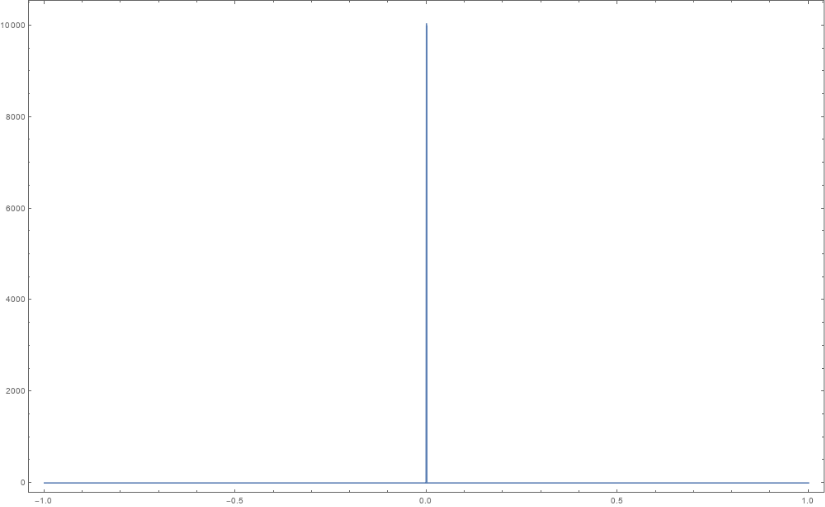
\includegraphics[scale=0.5]{delta-distribution.png}
	\caption{A Plot of $\delta(x)$}
\end{figure}
\section{Generalized Statistical Interpretation}
. \footnote{There of course exist other interpretations with subtle variations, we will discuss about these in Chapter \ref{epi}} If you measure an observable $\hat{O}$ on a particle in the state $\psi()$, you will certainly get one of the eigenvalues of the observable. If the spetra is discrete, the probability of getting the particular eigenvalue $q_{n}$ associated with the orthonormalized eigenfunction $f_{n}(x)$ is
\begin{equation}
	P(q_{n}) = \abs{c_{n}}^{2} = \abs{\braket{f_{x}}{\psi}}^{2}
\end{equation}
\subsection{Position Measurements}

\subsection{Momentum Measurements}

\section{Stationary State}
A  stationary state $\psi_{0}$ is a quantum mechanical state:
\begin{itemize}
\item with all observables independent of time
\item an eigenvector of the Hamiltonian
\item corresponds to a state with a single definite energy
\end{itemize}
Stationary states themselves are not constant in time but their probability densities $\abs{\psi_{0}}^{2}$ are
\section{The Continuity Equation}
\begin{tcolorbox}
\begin{equation}
\frac{\partial \rho}{\partial t} = - \nabla . \vec{J}
\end{equation}
\end{tcolorbox}
Where,
$$\rho = \psi \psi^{*}$$
$$\vec{J} = \frac{\hbar}{2mi} \left[ \psi^{*} \nabla \psi - (\nabla \psi^{*})\psi\right]$$
represents an interesting conservation law for quantum mechanics. But first, let's try to quickly prove this. 
\subsection{Proof}
W.k.t,
$$\frac{\partial}{\partial t}\int_{- \infty}^{\infty} \abs{\psi(\vec{x}, t)}^{2} dv = \frac{\partial}{\partial t}\int_{- \infty}^{\infty} \psi \psi^{*} dv = \int_{- \infty}^{\infty}  \psi^{*} \frac{\partial \psi}{\partial t} dv + \int_{- \infty}^{\infty}  \psi \frac{\partial \psi^{*}}{\partial t} dv = 0$$
\subsection{Interpretation}
\begin{itemize}
\item Probability is conserved i.e. $\sum_{i}^{\infty}P_{i} = 1$ \footnote{This holds well in the non-relativistic case i.e. when there is no creation or annihilation of particles}
\item The probability density evolves deterministically
\end{itemize}
\section{The Density Matrix}

\subsection{Properties}
\begin{itemize}
\item $\rho^{\dagger} = \rho$
\item$\Tr \rho= 1$
\item For a pure ensemble:
\begin{itemize}
\item $\rho^{2} = \rho$
\item $\Tr \rho^{2} \leq 1$
\end{itemize}
\item For an ensemble uniformly distributed over $k$ states: $\rho = (1/k)\mathbb{I}$
\end{itemize}
